\newcommand{\institut}{Institut f\"ur Energie und  Automatisiertungstechnik}
\newcommand{\fachgebiet}{Elektronische Mess- und Diagnosetechnik}
\newcommand{\veranstaltung}{Praktikum Messdatenverarbeitung}
\newcommand{\pdfautor}{\"Ozg\"u Dogan (326 048), Timo Lausen (325 411), Boris Henckell (325 779)}
\newcommand{\autor}{\"Ozg\"u Dogan (326 048)\\ Timo Lausen (325 411)\\ Boris Henckell (325 779)}
\newcommand{\pdftitle}{Praktikum Messdatenverarbeitung  Termin 1}
\newcommand{\prototitle}{Praktikum Messdatenverarbeitung \\ Termin 2}
\newcommand{\aufgabe}{}

\newcommand{\gruppe}{Gruppe: G1 Fr 08-10}
\newcommand{\betreuer}{Betreuer: J\"urgen Funk}

\input{../../packages/tu_header_8}
%---------------------------------------------------------------------
%---------------------------------------------------------------------
%---------------------------------------------------------------------

\section{Vorbereitungsaufgaben}
\begin{quote}
    \subsection{Sinusfunktion erzeugen und DFT erstellen}
    \begin{quote}
        siehe Quelltext sinus2.m im Anhang
        \begin{figure}[H]
        \centering
            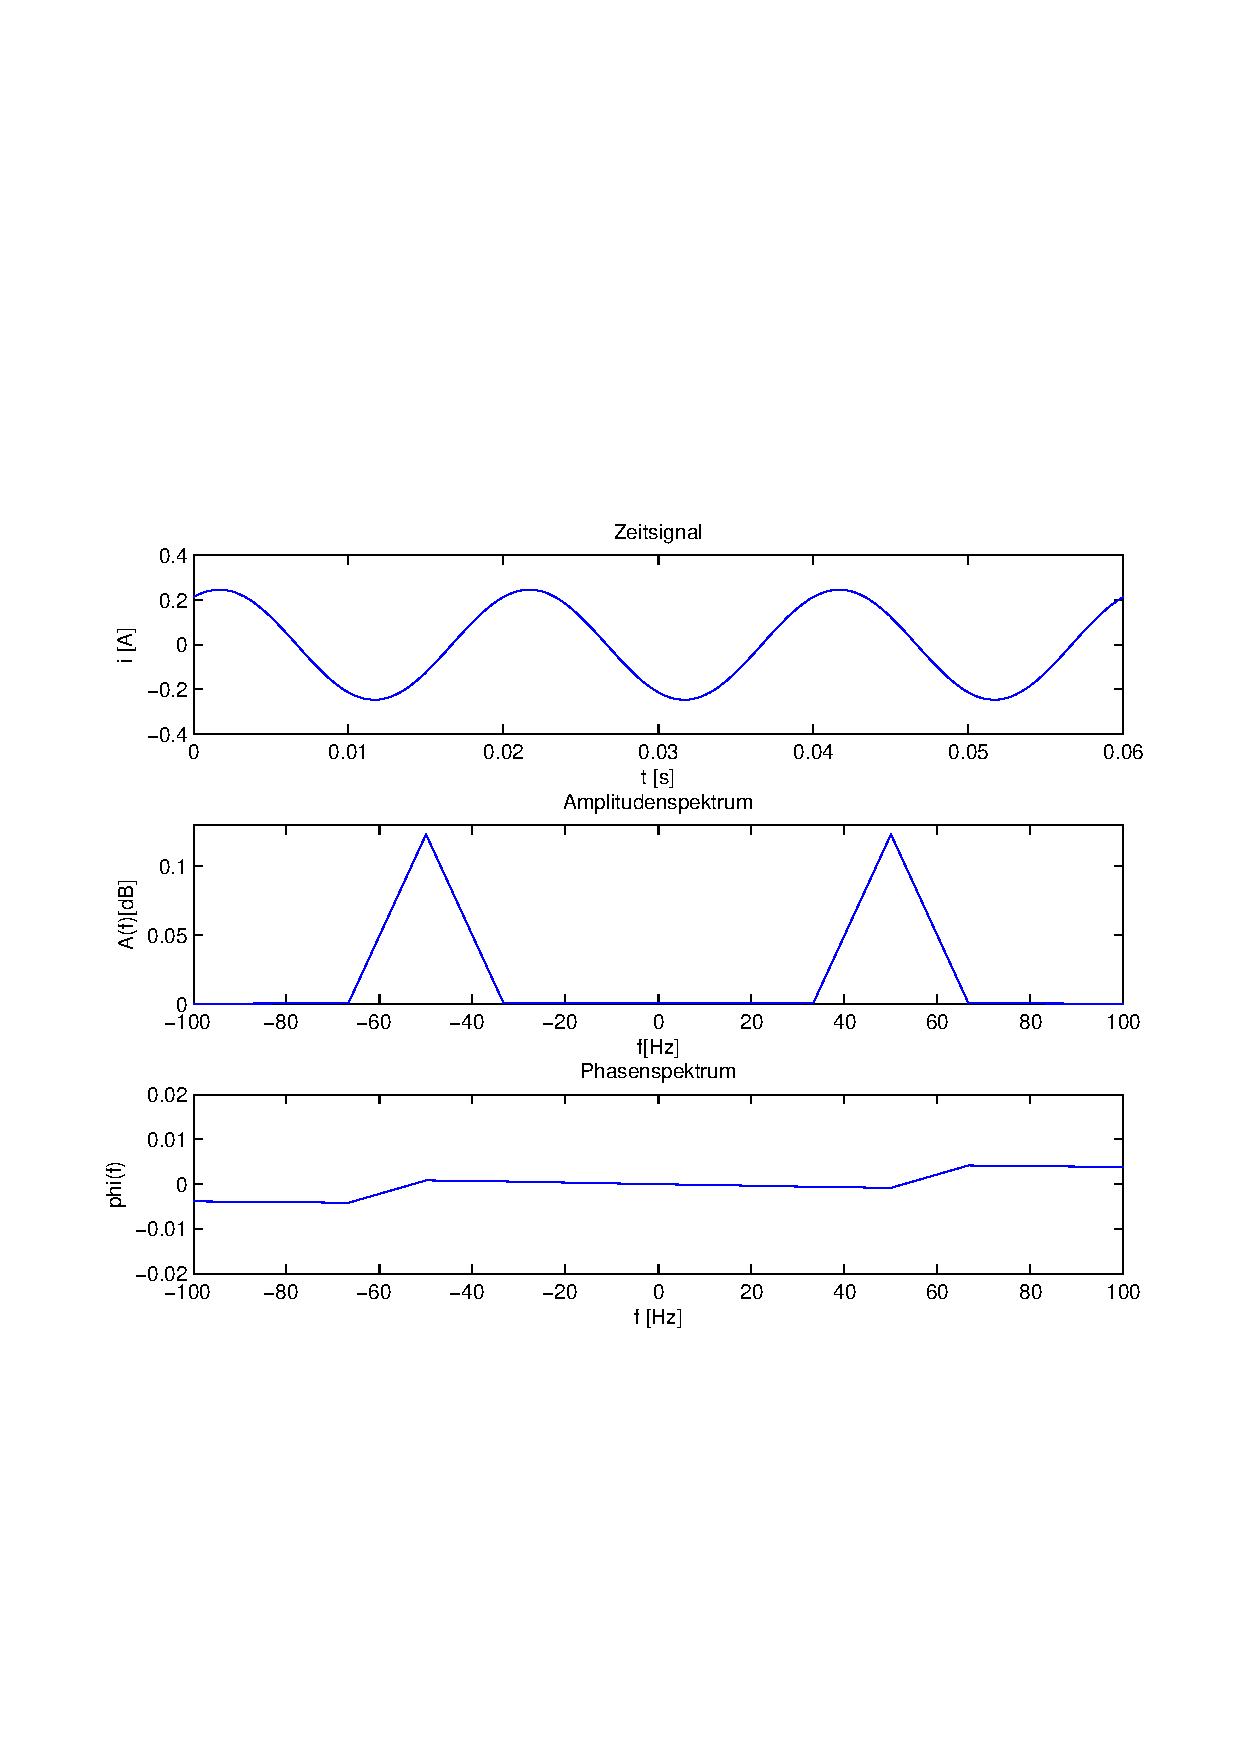
\includegraphics[scale=0.5, trim = 0cm 0cm 0cm 0cm, clip]{./Bilder/VerschobenerSinusAufgabe1}
                \caption{Verschobener Sinus}
                \label{fig:./Bilder/VerschobenerSinusAufgabe1}
        \end{figure}
    
    \end{quote}
    
	\subsection{Angeschnittene Sinusfunktion}
    \begin{quote}
        Siehe Quelltext stromPhasSchnitt.m im Anhang\\
        Um diese Funktion zu erstellen haben wir eine for Schleife imlementiert, die den gesamten zeitvektor t
        durchläuft. Für jeden Durchlauf wird getestet, wo sich der jeweilige Zeitpunkt im Verhältniss zum halben
        sinussignal befindet. Anschließend wird in der if abfrage bestimmt, ob sich dieser Zeitpunkt relativ zur halben
        Periode des Sinussignals vor oder hinter dem Phasenanschnittswinkel befindet. Abhängig davon wird der
        dentsprechenden Stelle im Ausgabevektor der Wert $0$ oder der Wert den die Sinusfunktion ermittelt, übergeben.\\
        Für die Phasenanschnittswinkel. $ \alpha = 0, \frac{1}{8} \pi, \frac{1}{4} \pi, \frac{3}{8} \pi, \frac{1}{2}
        \pi,\frac{5}{8} \pi, \frac{3}{4} \pi, \frac{7}{8} \pi$ und $\pi$ ergeben sich folgende 
    \end{quote}
    
    \subsection{Effektivwert des Stroms im Zeitbereich}
    \begin{quote}
        Siehe Quelltext EffektivwertZeitbereich.m im Anhang\\
        Für den Effektivwert des Stroms im Zeitbereich ermitteln wir die Wurzel des Mittelwertes des Quadrats des
        Stromvektors.
    \end{quote}
    
    \subsection{Effektivwert des Stroms im Frequenzbereich}
    \begin{quote}
        Siehe Quelltext EffektivwertFourier.m im Anhang\\
        Den Effektivwert des Stroms im Frequenzbereich ermitteln wir ähnlich wie den Effektivwert des Stroms im
        Zeitbereich. Dank des Parsevalschen-Theorems \ldots
        \end{quote}
    \subsection{Ergebnisse Vorbereitungsaufgaben}
    \begin{quote}
                                %4 Grafiken:
            \begin{center}
            \begin{tabular}{ll}

            \hspace{-4em}
                \begin{minipage}{0.6\textwidth}

                    \begin{figure}[H]
                        \label{fig:}
                        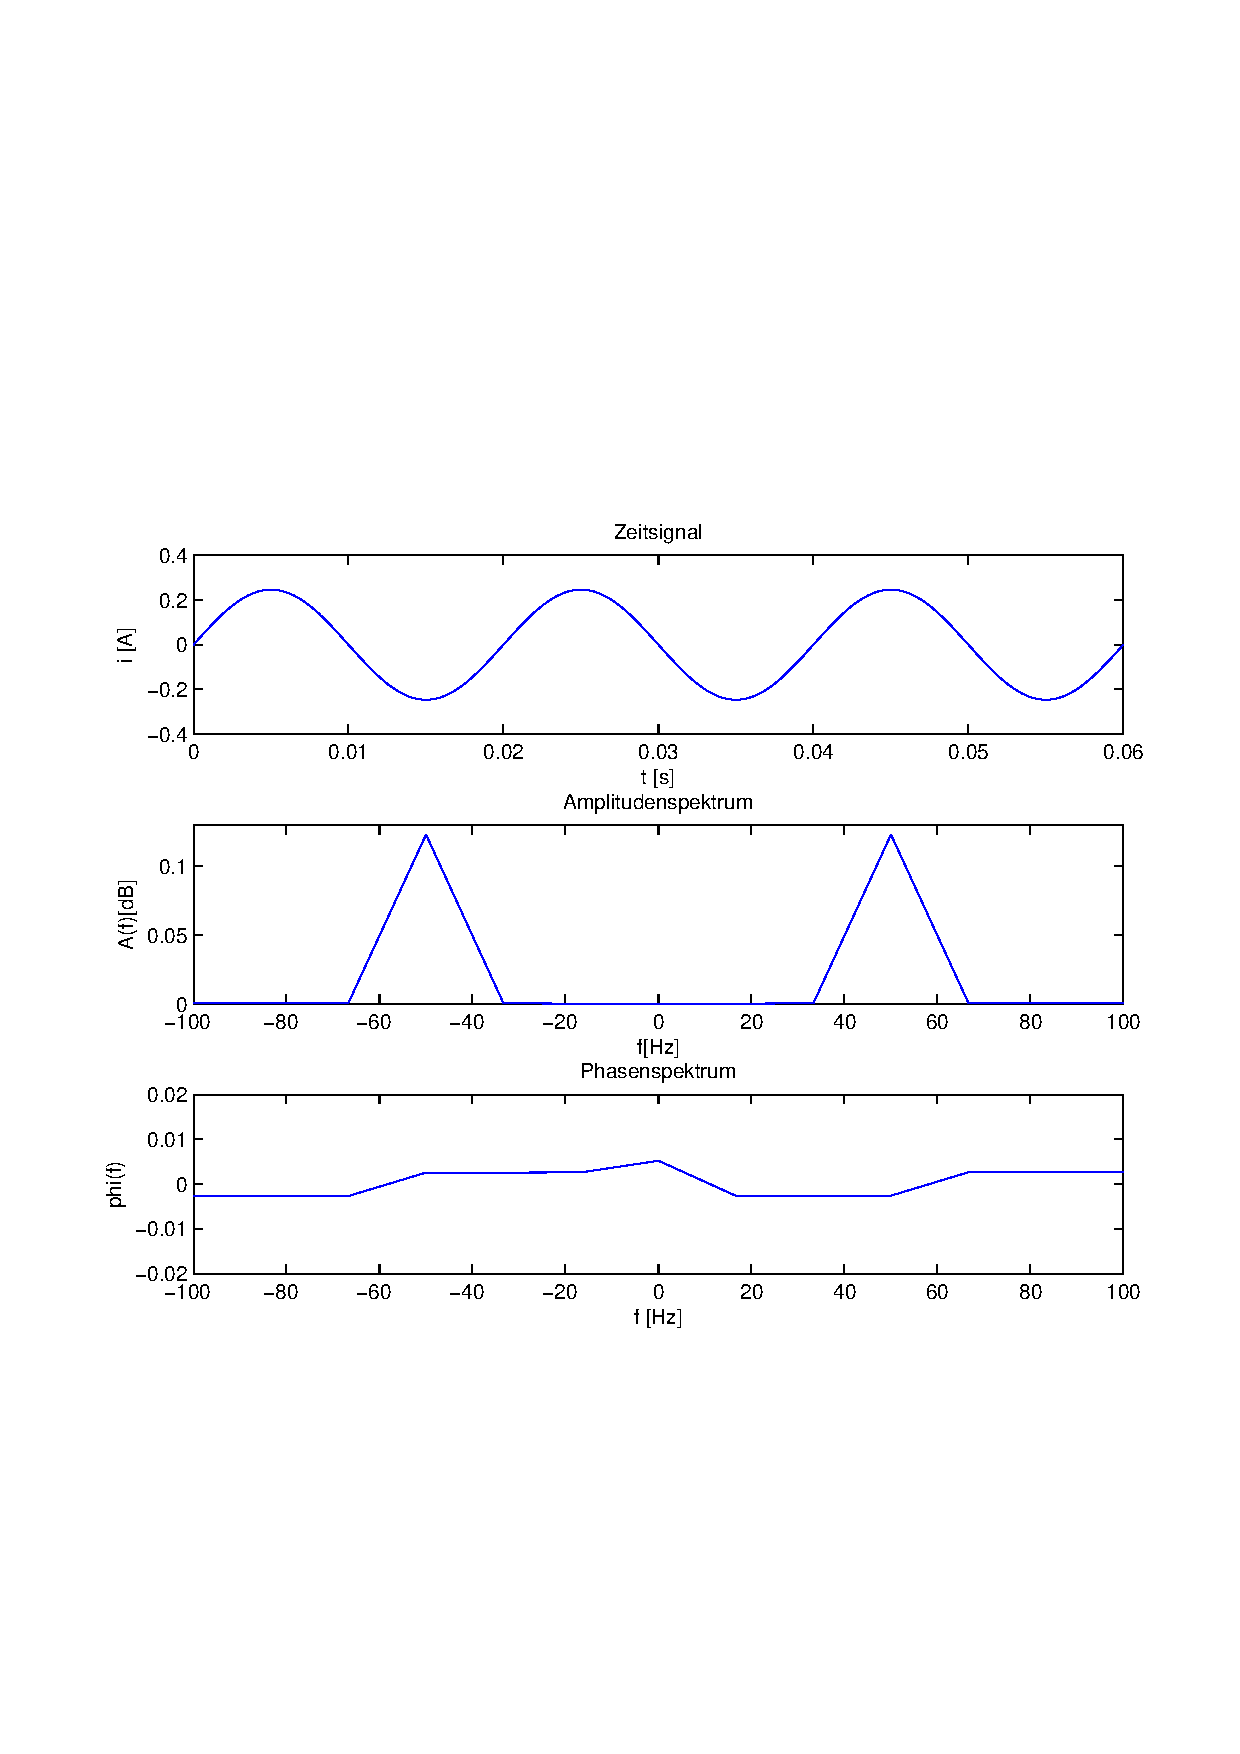
\includegraphics[scale=0.3]{./Bilder/Phasenanschnitt08pi.pdf} %FIXME [width=640px,
                         %height=474px]
                        \caption{Sinussignal mit Phasenanschnitt von $0$}
                    \end{figure}

                \end{minipage}
                \begin{minipage}{0.6\textwidth}

                    \begin{figure}[H]
                        \label{fig:}
                        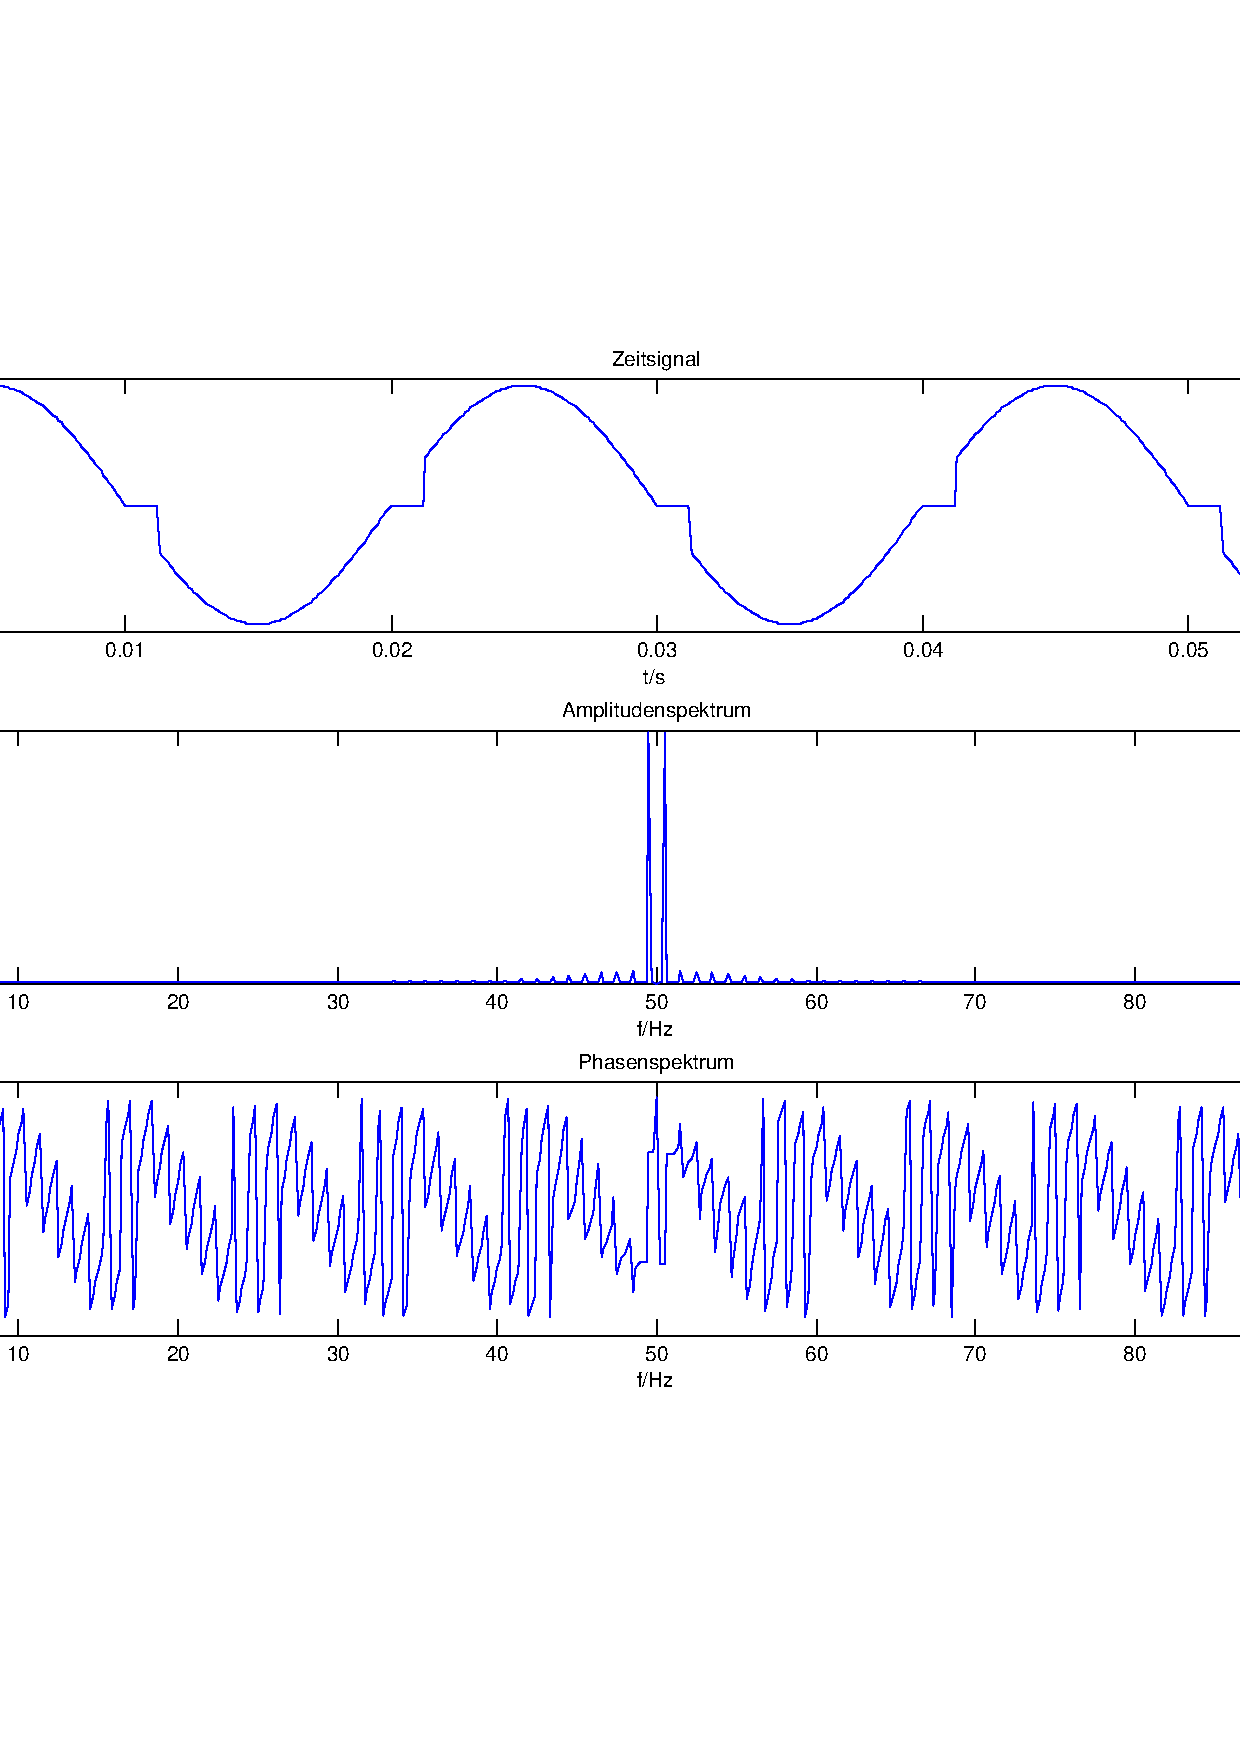
\includegraphics[scale=0.3]{./Bilder/Phasenanschnitt18pi.pdf} %FIXME [width=640px,
                         %height=474px]
                        \caption{Sinussignal mit Phasenanschnitt von $\frac{1}{8}/pi$}
                    \end{figure}
                \vspace{-1.5em}

                \end{minipage}

            \end{tabular}
            \end{center}

                        %4 Grafiken:
            \begin{center}
            \begin{tabular}{ll}

            \hspace{-4em}
                \begin{minipage}{0.6\textwidth}

                    \begin{figure}[H]
                        \label{fig:}
                        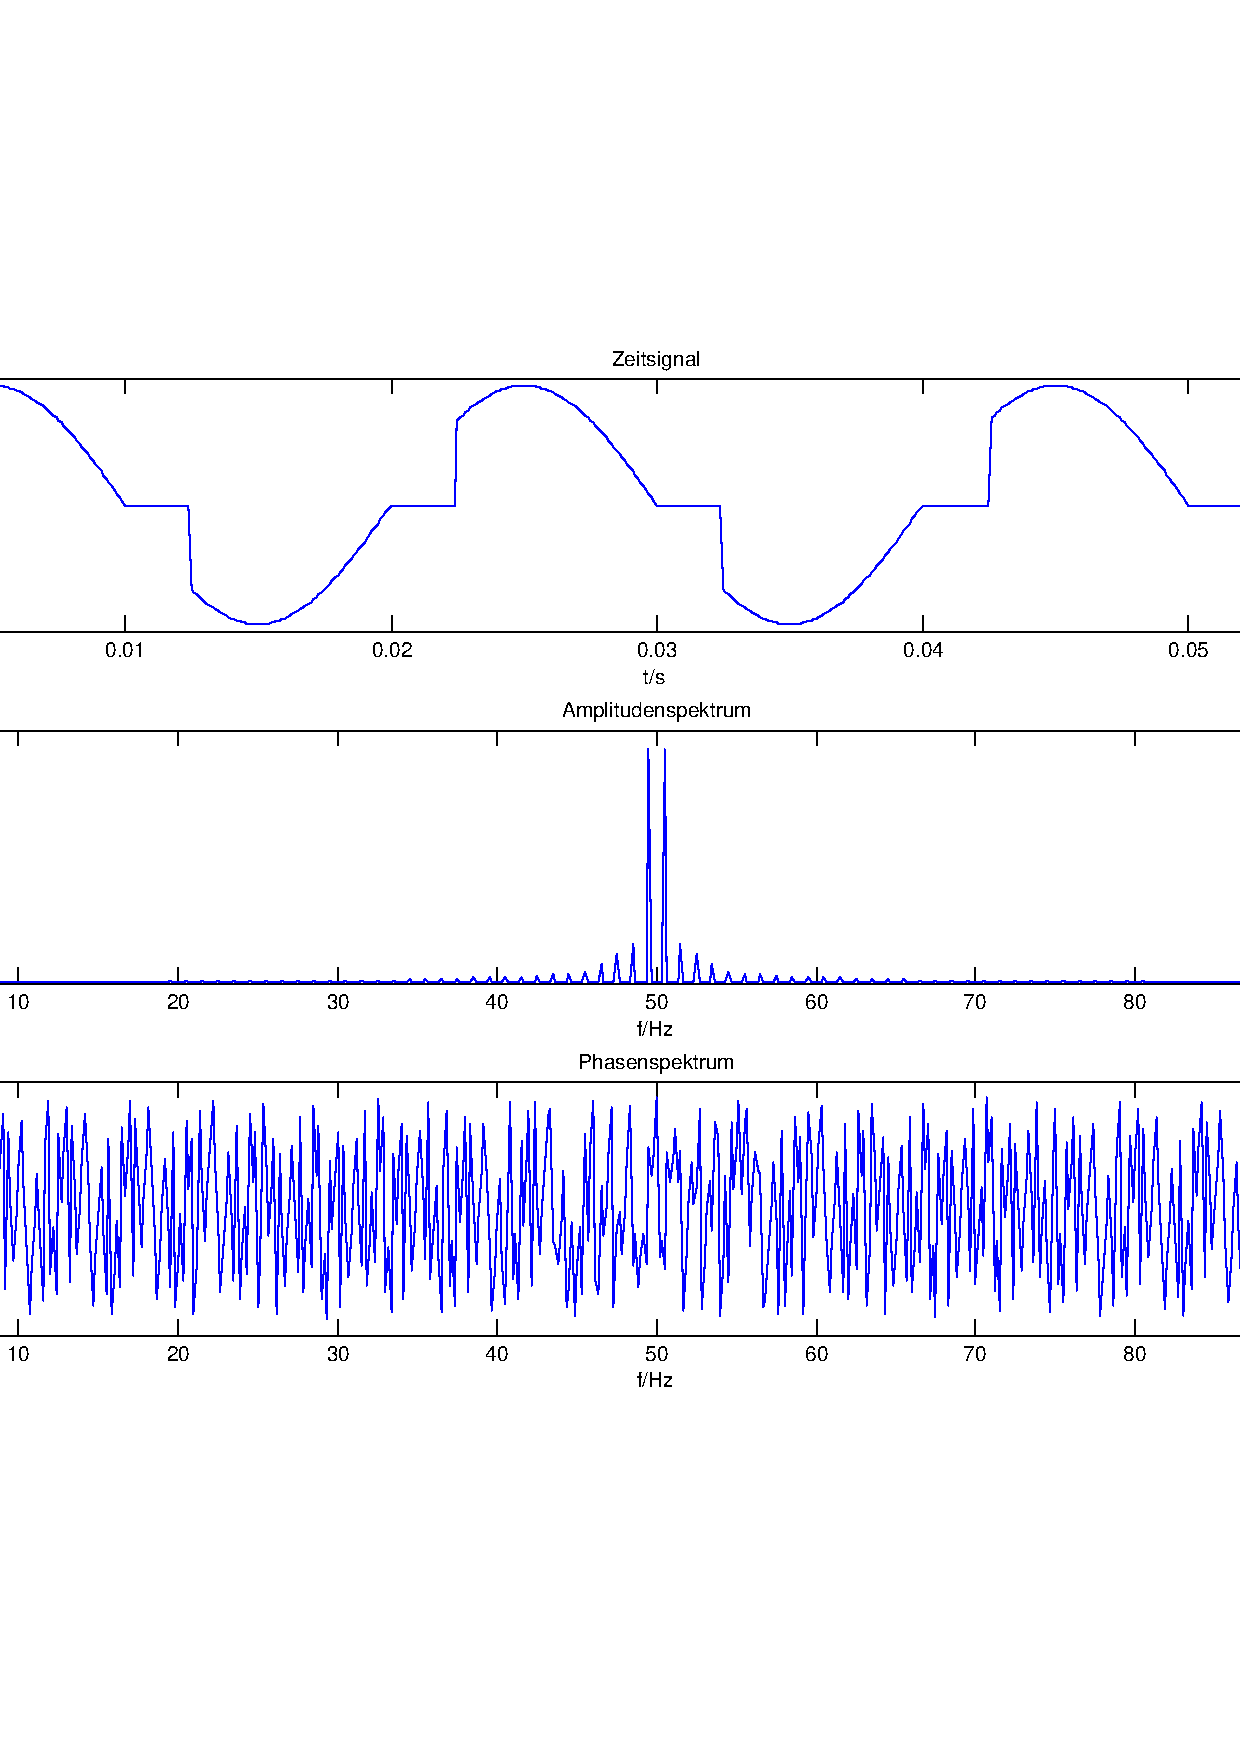
\includegraphics[scale=0.3]{./Bilder/Phasenanschnitt28pi.pdf} %FIXME [width=640px,
                        % height=474px]
                        \caption{Sinussignal mit Phasenanschnitt von $\frac{1}{4}/pi$}
                    \end{figure}

                \end{minipage}
                \begin{minipage}{0.6\textwidth}

                     \begin{figure}[H]
                        \label{fig:}
                        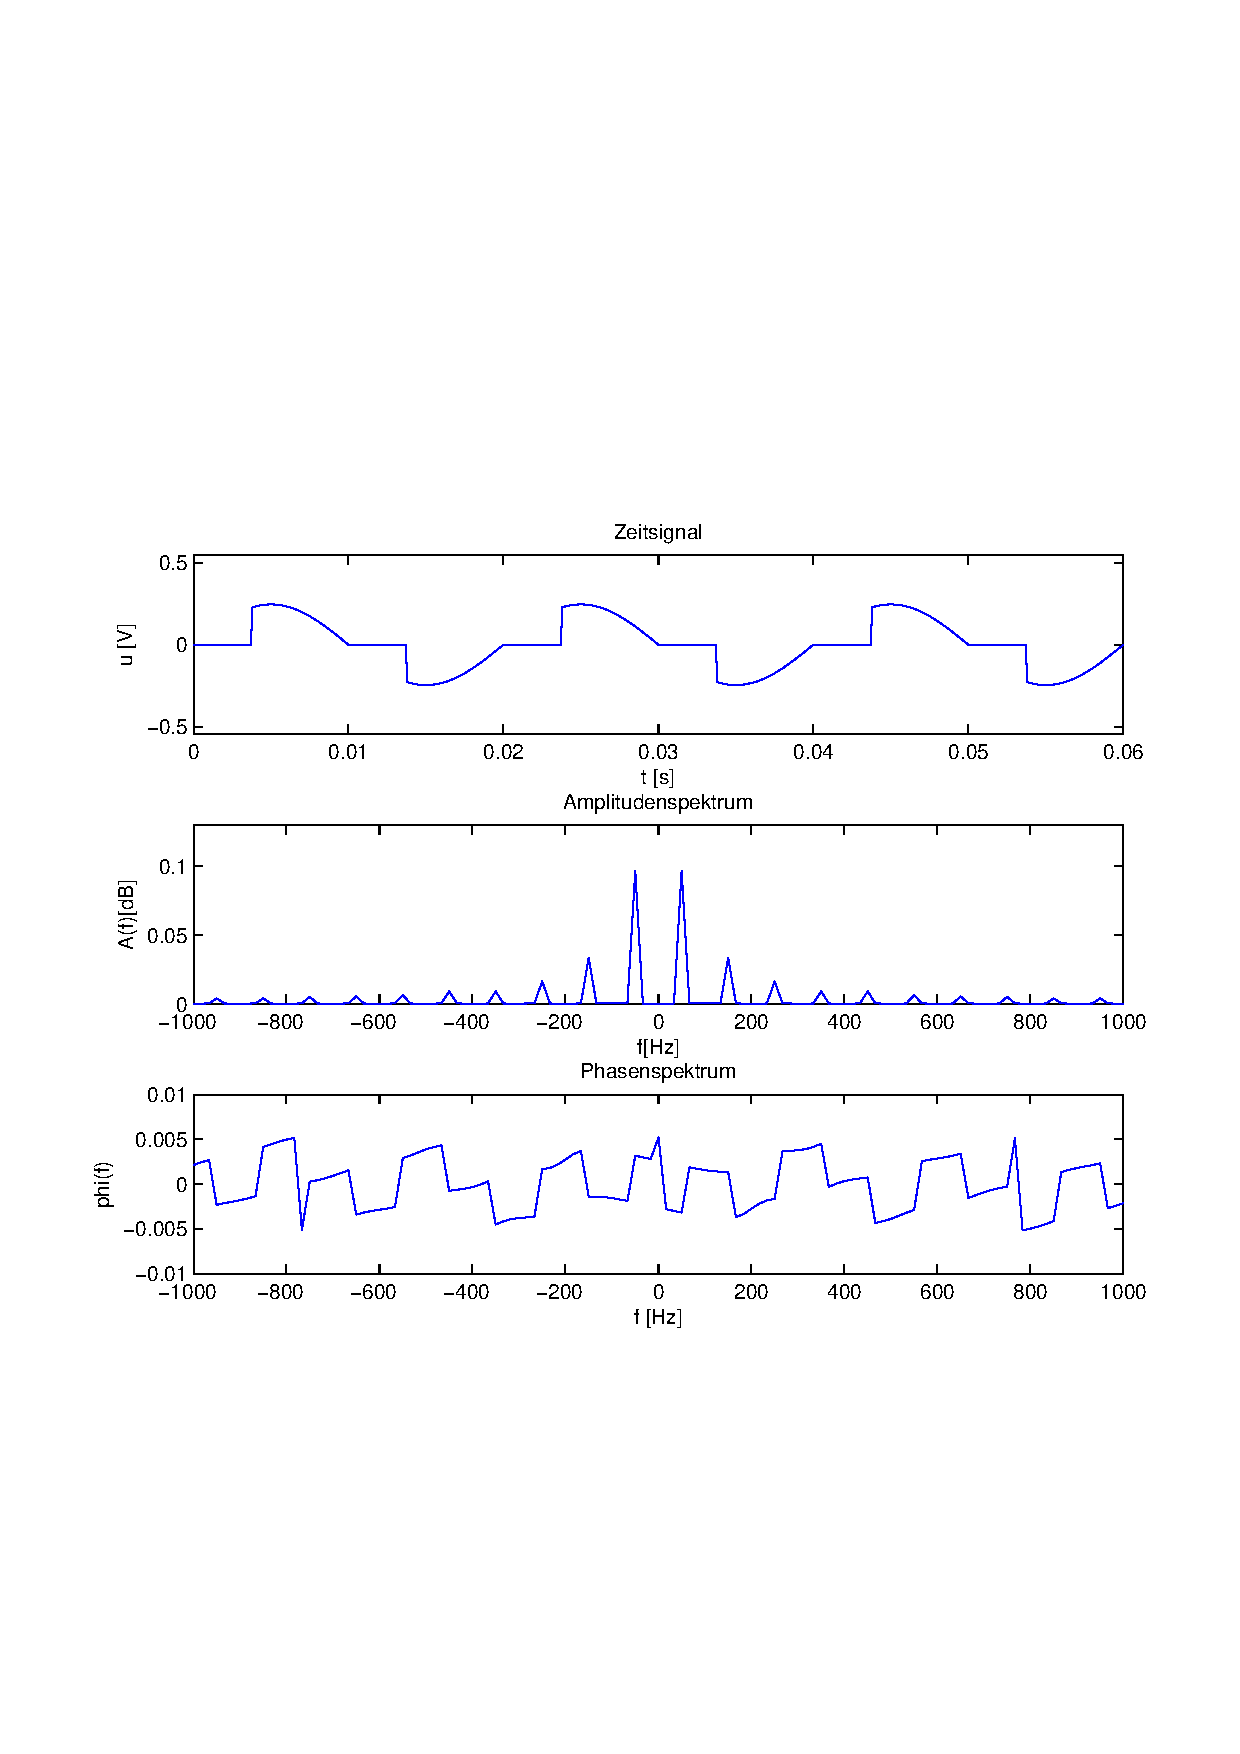
\includegraphics[scale=0.3]{./Bilder/Phasenanschnitt38pi.pdf} %FIXME [width=640px,
                        % height=474px]
                        \caption{Sinussignal mit Phasenanschnitt von $\frac{3}{8}/pi$}
                    \end{figure}
               \vspace{-1.5em}

                \end{minipage}

            \end{tabular}
            \end{center}

                        %4 Grafiken:
            \begin{center}
            \begin{tabular}{ll}

            \hspace{-4em}
                \begin{minipage}{0.6\textwidth}

                    \begin{figure}[H]
                        \label{fig:}
                        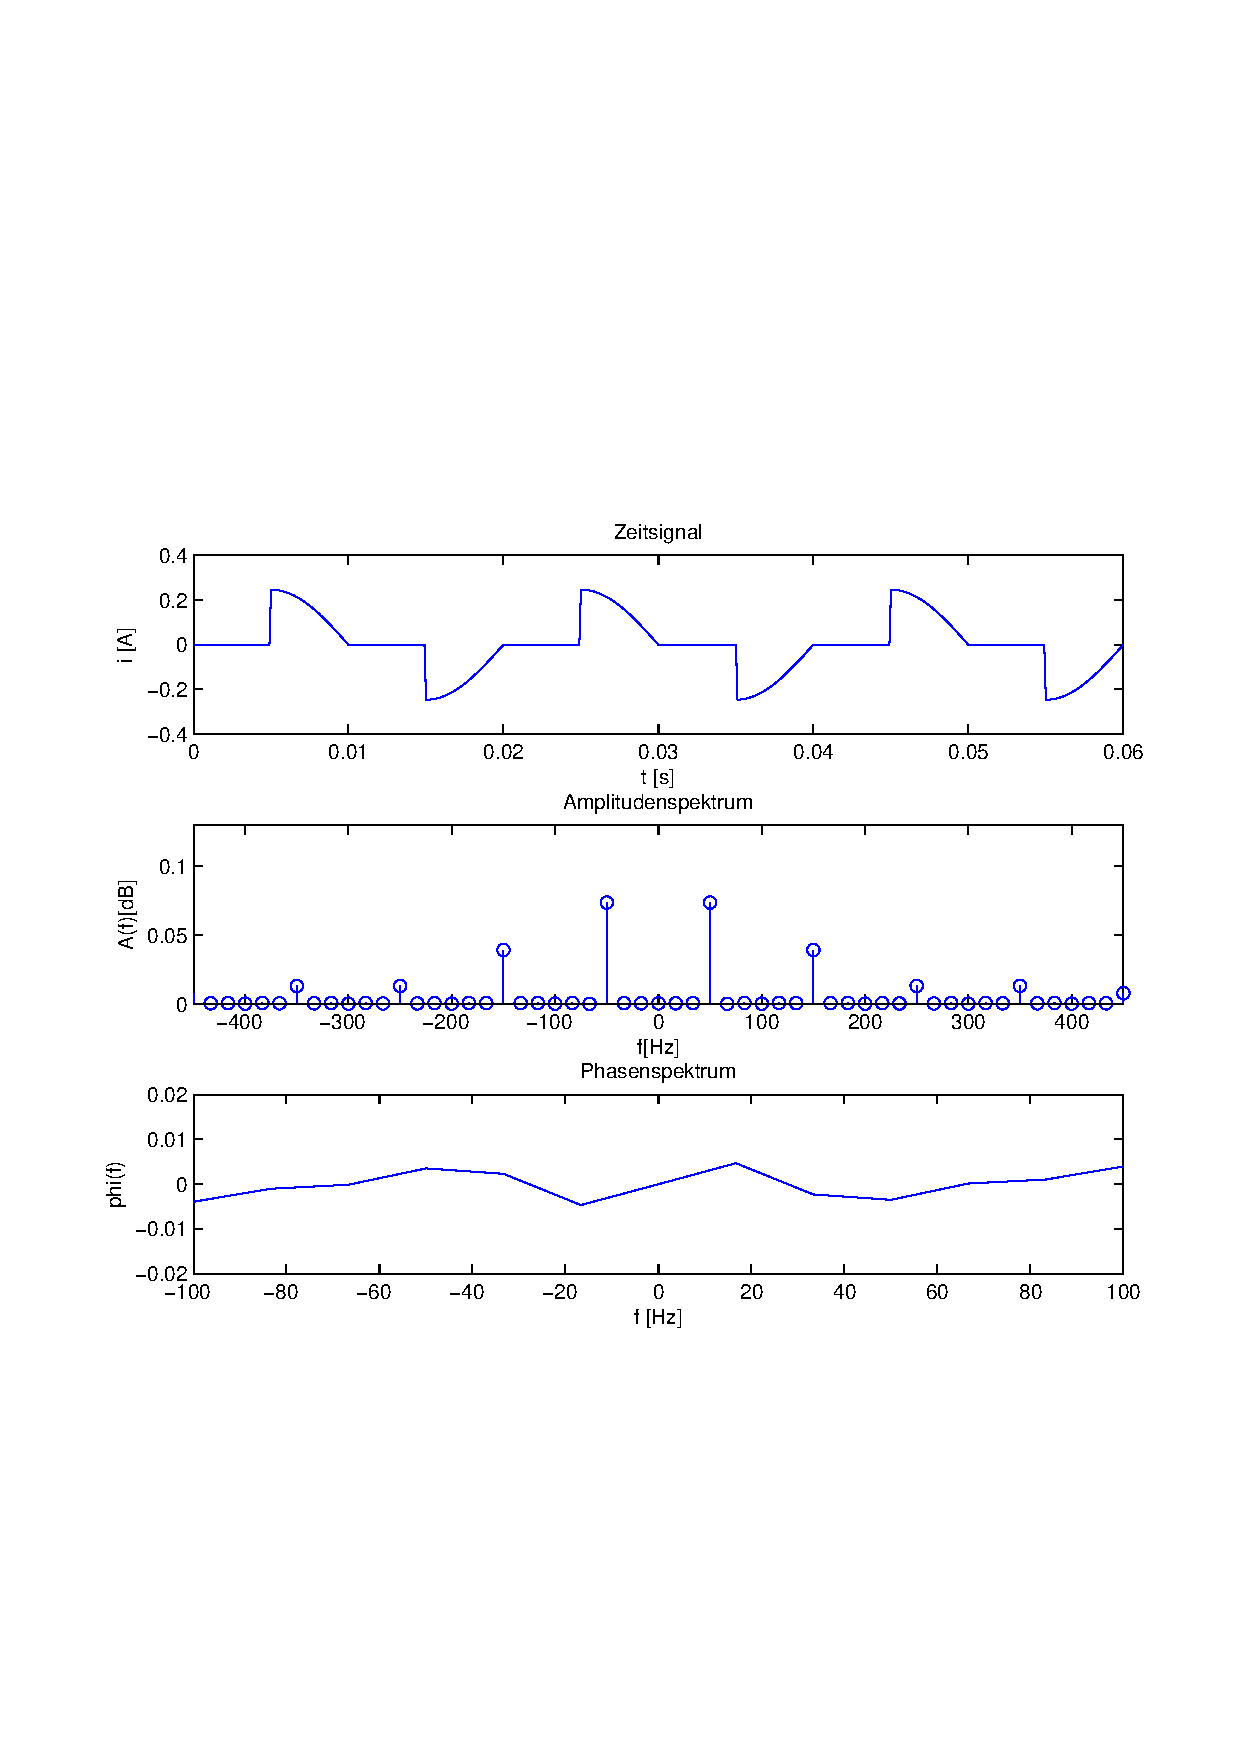
\includegraphics[scale=0.3]{./Bilder/Phasenanschnitt48pi.pdf} %FIXME [width=640px,
                        % height=474px]
                        \caption{Sinussignal mit Phasenanschnitt von $\frac{1}{2}/pi$}
                    \end{figure}

                \end{minipage}
                \begin{minipage}{0.6\textwidth}

                   \begin{figure}[H]
                        \label{fig:}
                        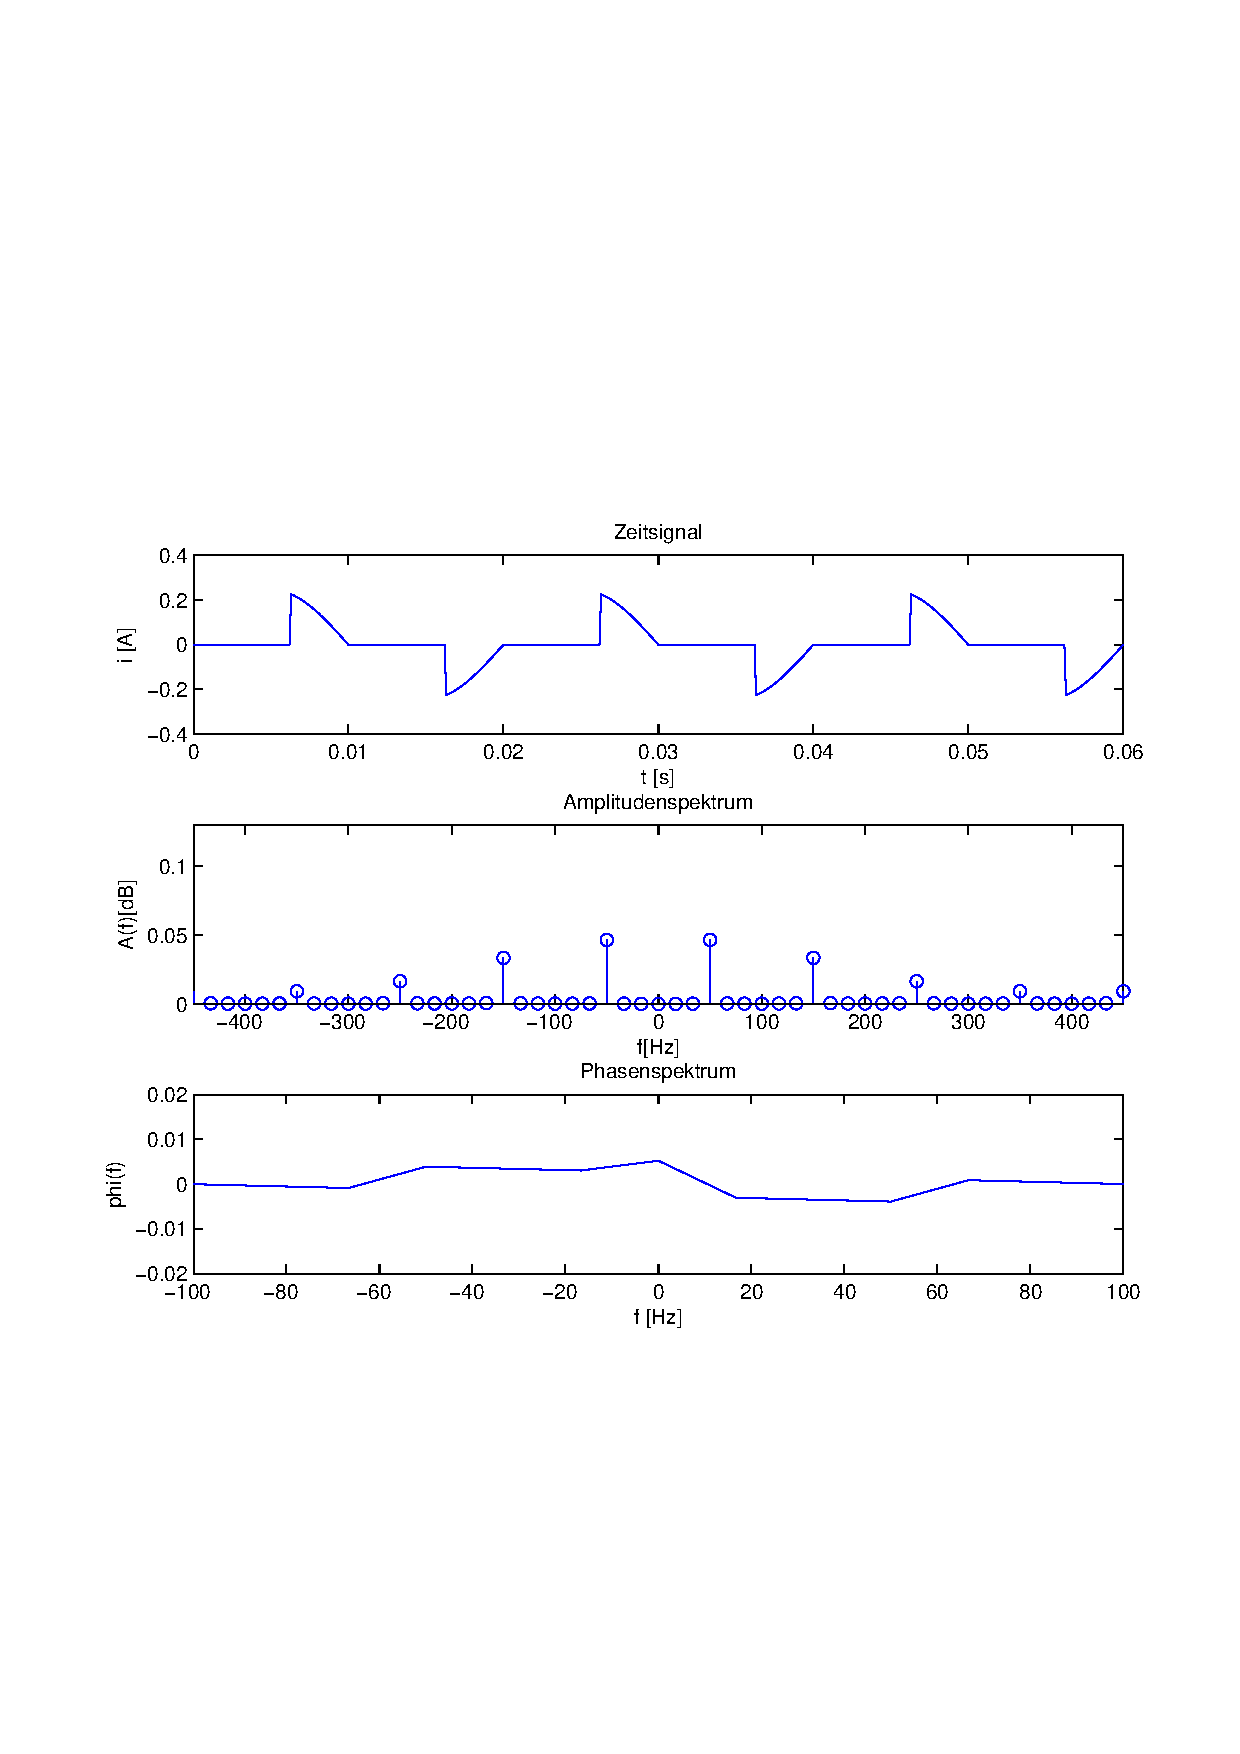
\includegraphics[scale=0.3]{./Bilder/Phasenanschnitt58pi.pdf} %FIXME [width=640px,
                        % height=474px]
                        \caption{Sinussignal mit Phasenanschnitt von $\frac{5}{8}/pi$}
                    \end{figure}
                 \vspace{-1.5em}

                \end{minipage}

            \end{tabular}
            \end{center}

               %4 Grafiken:
            \begin{center}
            \begin{tabular}{ll}

            \hspace{-4em}
                \begin{minipage}{0.6\textwidth}

                    \begin{figure}[H]
                        \label{fig:}
                        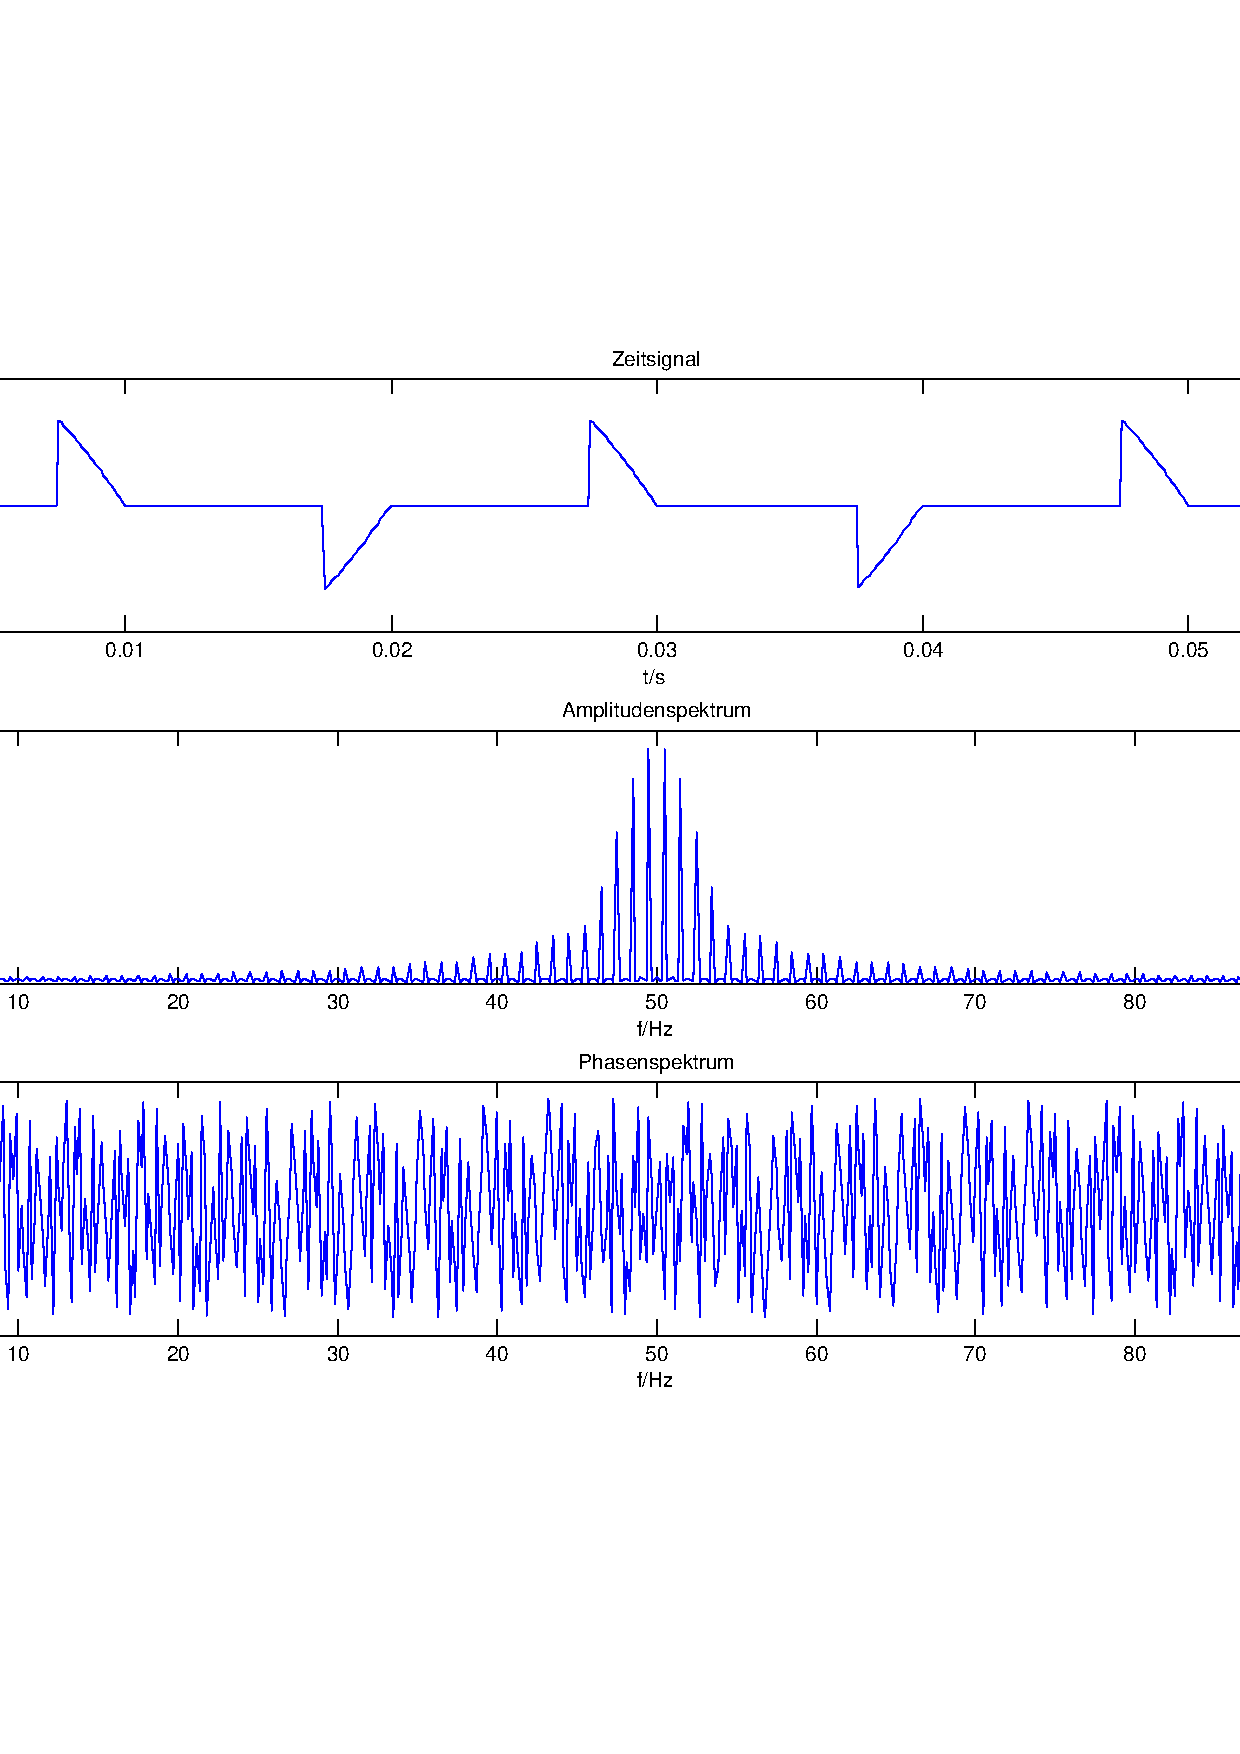
\includegraphics[scale=0.3]{./Bilder/Phasenanschnitt68pi.pdf} %FIXME [width=640px,
                        % height=474px]
                        \caption{Sinussignal mit Phasenanschnitt von $\frac{3}{4}/pi$}
                    \end{figure}

                \end{minipage}
                \begin{minipage}{0.6\textwidth}

                   \begin{figure}[H]
                        \label{fig:}
                        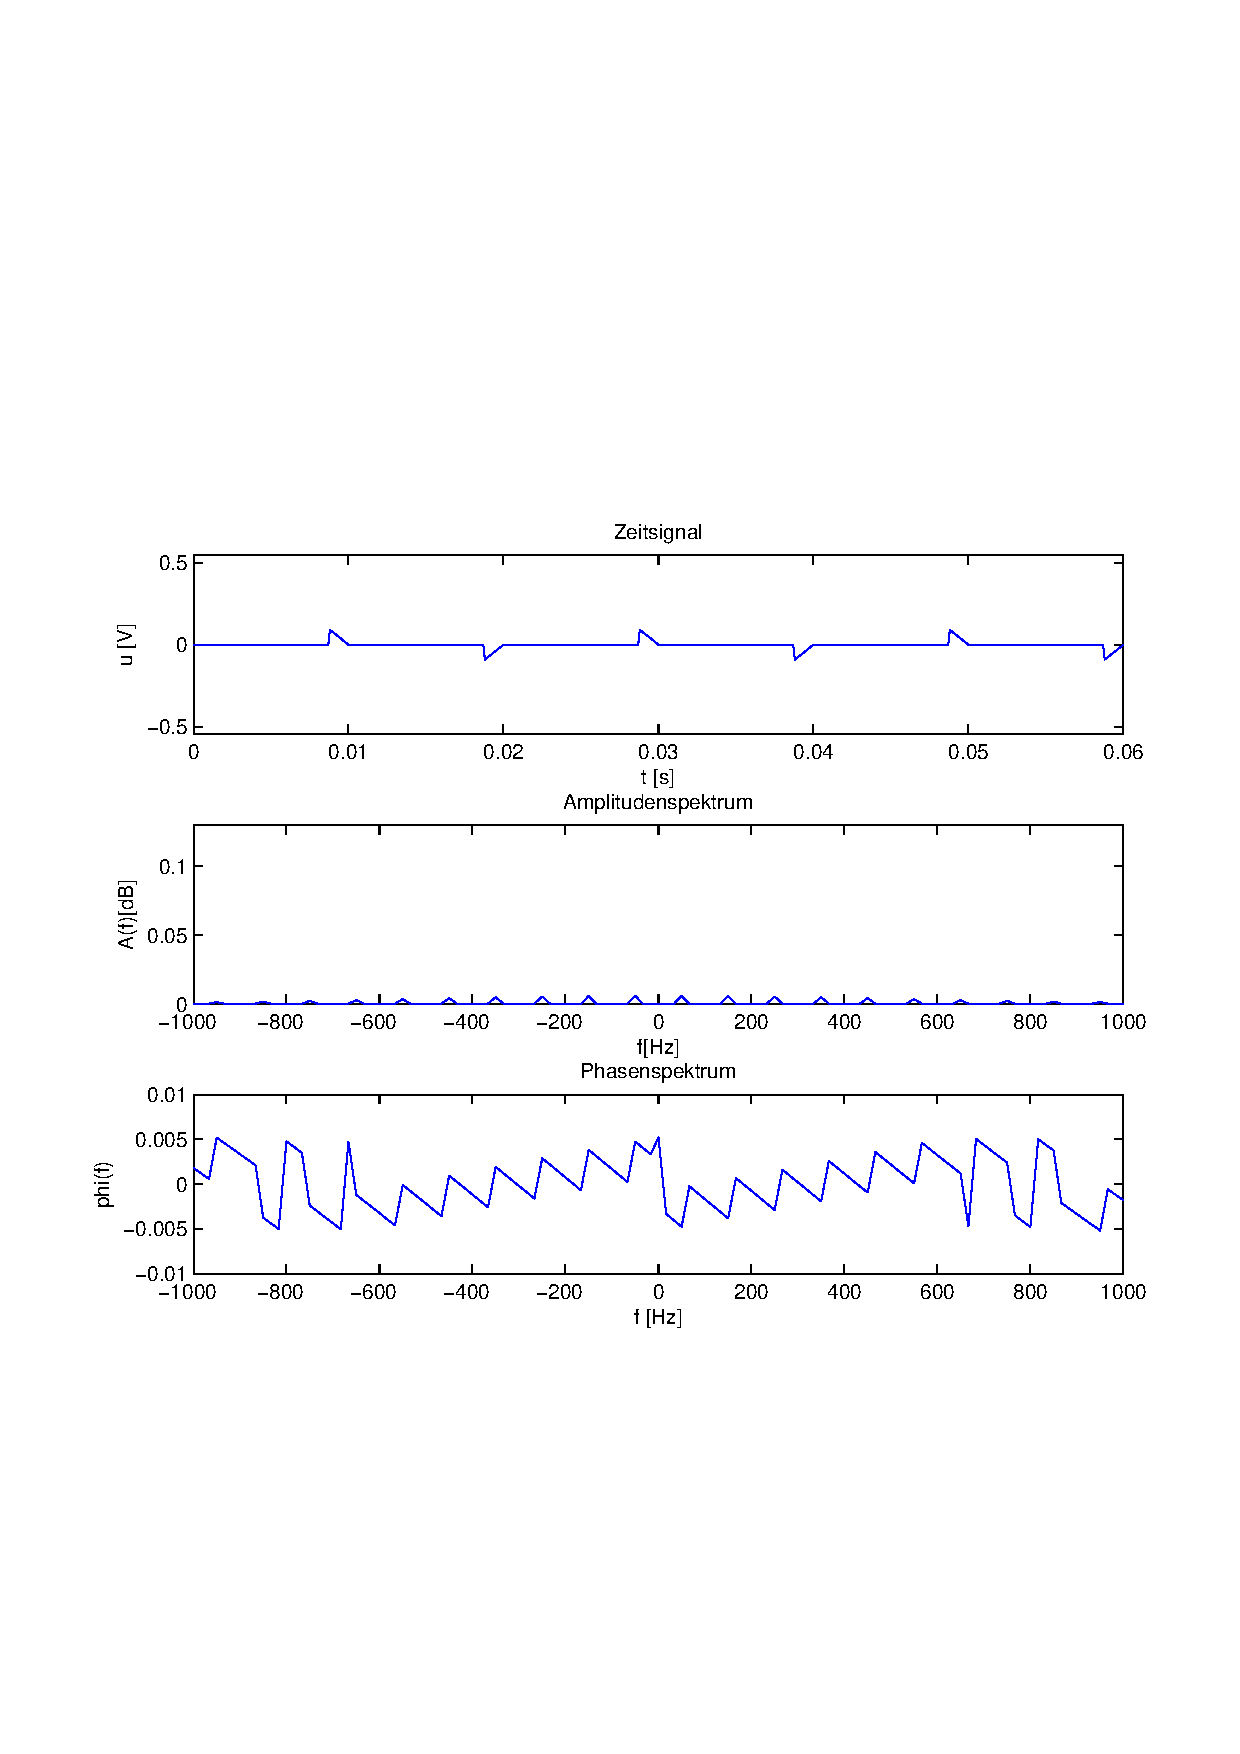
\includegraphics[scale=0.3]{./Bilder/Phasenanschnitt78pi.pdf} %FIXME [width=640px,
                        % height=474px]
                        \caption{Sinussignal mit Phasenanschnitt von $\frac{7}{8}/pi$}
                    \end{figure}
                 \vspace{-1.5em}

                \end{minipage}

            \end{tabular}
            \end{center}
            
               %4 Grafiken:
            \begin{center}
            \begin{tabular}{ll}

            \hspace{-4em}
                \begin{minipage}{0.6\textwidth}

                    \begin{figure}[H]
                        \label{fig:}
                        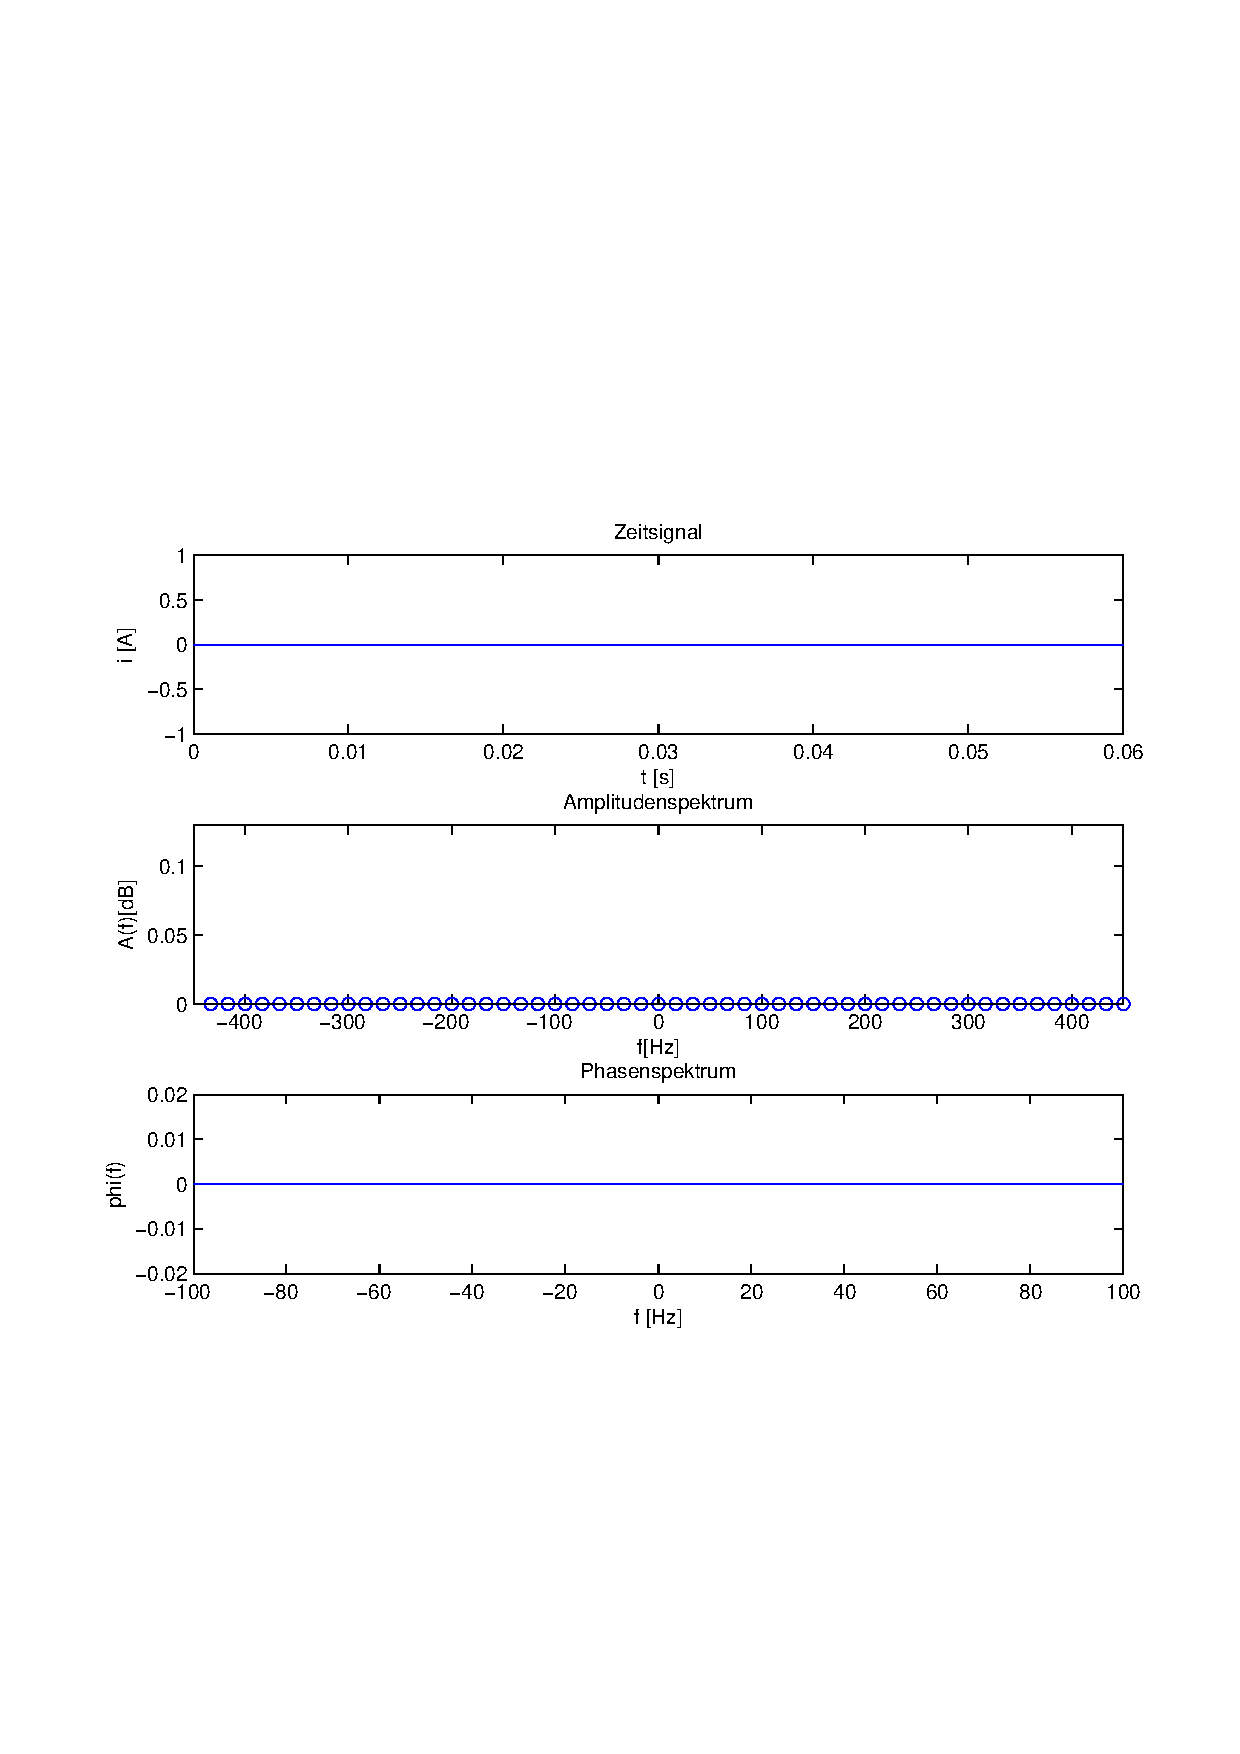
\includegraphics[scale=0.3]{./Bilder/Phasenanschnitt88pi.pdf} %FIXME [width=640px,
                        % height=474px]
                        \caption{Sinussignal mit Phasenanschnitt von $/pi$}
                    \end{figure}

                \end{minipage}

            \end{tabular}
            \end{center}
             \begin{center}
                 \begin{tabular}{|c|c|c|}
                             
                   \hline
                   $\alpha $ & $i_{eff}$ (Zeitbereich) & $i_{eff}$ Frequenzbereich\\ \hline
                   $0$ & 3,5326 & 3,5326 \\ \hline
                   $\frac{1}{8} \pi$ & 3,5105 & 3,5105 \\ \hline
                   $\frac{1}{4} \pi$ & 3,3744 & 3,3744 \\ \hline
                   $\frac{3}{8} \pi$ & 3,0338 & 3,0338 \\ \hline
                   $\frac{1}{2} \pi$ & 2,5145 & 2,5145 \\ \hline
                   $\frac{5}{8} \pi$ & 1,8097 & 1,8097 \\ \hline
                   $\frac{3}{4} \pi$ & 1,0748 & 1,0748 \\ \hline
                   $\frac{7}{8} \pi$ & 0,3940 & 0,3940 \\ \hline
                   $ \pi$ & 0 & 0 \\ \hline
                         
           
                 \end{tabular}
             \end{center}        
        
        
    \end{quote}
\end{quote}

%--------------------------------------------------------------------
%--------------------------------------------------------------------

\section{Versuch}
\begin{quote}
	
\end{quote}

%--------------------------------------------------------------------
%--------------------------------------------------------------------

\section{Ergebnisse}
\begin{quote}
	
\end{quote}

%--------------------------------------------------------------------
%--------------------------------------------------------------------
\section{Quellcode}
\begin{quote}
    \subsection{sinus2.m}
    \begin{quote}
        \lstinputlisting[
            caption={sinus2},
            label=lst:Matlab]
            {./Matlab/sinus2.m}
    \end{quote}
    \subsection{stromPhasSchnitt.m}
    \begin{quote}
        \lstinputlisting[
            caption={stromPhasSchnitt},
            label=lst:Matlab]
            {./Matlab/stromPhasSchnitt.m}
    \end{quote}
    \subsection{EffektivwertZeitbereich.m}
    \begin{quote}
        \lstinputlisting[
            caption={EffektivwertZeitbereich},
            label=lst:Matlab]
            {./Matlab/EffektivwertZeitbereich.m}
    \end{quote}
    \subsection{EffektivwertFourier.m}
    \begin{quote}
        \lstinputlisting[
            caption={EffektivwertFourier},
            label=lst:Matlab]
            {./Matlab/EffektivwertFourier.m}
    \end{quote}
	
\end{quote}

%--------------------------------------------------------------------
%--------------------------------------------------------------------


\begin{thebibliography}{999}
%\bibitem {DigitaleMesskette} Prof. Dr.-Ing. Gühmann, Clemens: MDVScript\_01, S.5

%Name, Vorname.; evtl. Name2, Vorname2.: Titel des Dokumentes
%oder Buches, Zeitschrift/Verlag/URL (Auflage, Erscheinungsort, -jahr), ggf. Seitenzahlen
%\bibitem [Wiki10] {DigitaleMesskette2} \url{www.wikipedia.org}, Zugriff 22.03.2010
\end{thebibliography}


\end{document}


